\chapter{Conceptual Approach}
\label{chap:conceptual-approach}
The goal of this chapter is to derive some precise requirements for the design of a system that can facilitate the sharing of Cyber Threat Intelligence (CTI) in a decentralized manner. This will lay the foundation for the realization of the objectives of this research. To achieve this, we will first discuss our methodology to reach our objectives which is based on design science methodology. We will then try to understand the missing pieces in the current systems that prevent the sharing of CTI in a decentralized manner which is the concept of data sovereignty. We will then discuss the alternative approaches to achieve data sovereignty. Then, we will look at some real-world scenarios where CTI sharing is challenging. Following that, we will derive high-level requirements for a system with the chosen approach. Finally, we will discuss the conceptual approach to achieve these requirements.

% 12 Pages
\section{Methodology}
In this section, we describe the methodology used in this research. In doing so, we start with a brief introduction to the Design Science Research (DSR) methodology. We then explain how we plan to use this methodology to achieve the objectives of this research.

% - design science
\subsection{Design Science Research (DSR)}
Design Science Research (DSR) is a research methodology that aims to create and evaluate artifacts to solve real-world problems in the context of Information Systems research \cite{hevner_three_2007}. Our research is also heavily inspired by this approach. Hevner defines a three cycle view of DSR, which consists of relevance, rigor, and design in an inspiring article \cite{hevner_three_2007}. A good DSR research should have adequate progress in each cycle. 
\subsubsection{Relevance}
The relevance cycle tries to keep the design research activities relevant to its application's domain. Therefore it involves understanding the problem domain, the stakeholders, the limitations of current systems. It should elicit the requirements to form the basis of the expectencies from the resulting artifact. After the artifact is created, it should be evaluated in terms of its relevance to the problem domain. This take place multiple rounds until the artifact is deemed relevant enough.
\subsubsection{Rigor}
The rigor cycle is aimed at ensuring the scientific rigor of the research. This involves grounding the design methods in the existing literature, using appropriate scientific methods. It requires systematically reviewing the existing literature to ensure that the research is innovative. At the end of each cycle, the findings should be shared with the scientific community to get feedback.
\subsubsection{Design}
The design cycle is the core of the DSR methodology. It involves creating the artifact that solves the problem. It should be based on the input from the former two cycles, namely the requirements and the scientific methods. Each produced artifact should be evaluated appropriately to ensure that it meets the requirements. 

A summary of the DSR methodology is shown in Figure \ref{fig:dsr-cycle}.

\begin{figure}[ht]
    \centering
    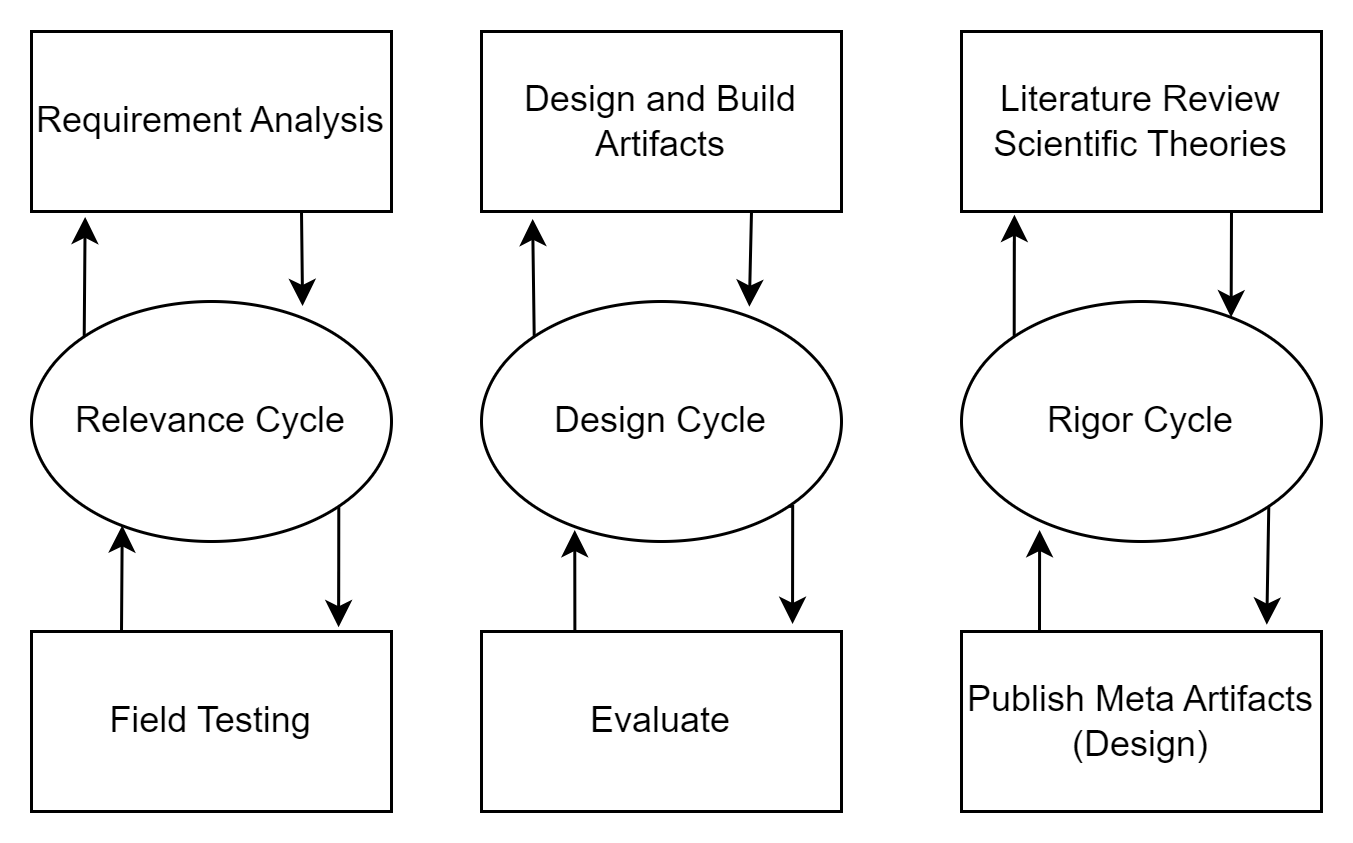
\includegraphics[width=0.8\textwidth]{diagrams/conceptual/dsr-cycle.png}
    \caption{Design Science Research Cycle \cite{hevner_three_2007}}
    \label{fig:dsr-cycle}
\end{figure}

% - how we plan to use DSR
\subsection{Application of DSR in this Research}
Our methodology is heavily inspired by the DSR methodology.
It comprises of two main phases that each consist of multiple iterations.
The first phase is the inception phase, where the goal is to understand the main challenges in designing of CTI Dataspace and a conceptual approach of the system.
In this phase we try to find specific gaps in the current CTI sharing schemes that could be addressed by a Dataspace based solution.
To do so, we delve into the current CTI sharing scenarios by looking at the existing platforms, the scientific literature, and some guidelines and regulations.
The next step in this phase is to collect as much as possible information about the Dataspace concept, its promises, and its use cases.
The subsequent step is to leverage the information gathered in the previous steps to find improvement areas that could be addressed by a Dataspace based solution. After several iterations, we will have a high level understanding of the design of a Dataspace based CTI sharing platform and a real-world scenario where it could highlight its advantages over traditional CTI sharing platforms. This phase is summarized in Figure \ref{fig:inception-phase}.

\begin{figure}[ht]
    \centering
    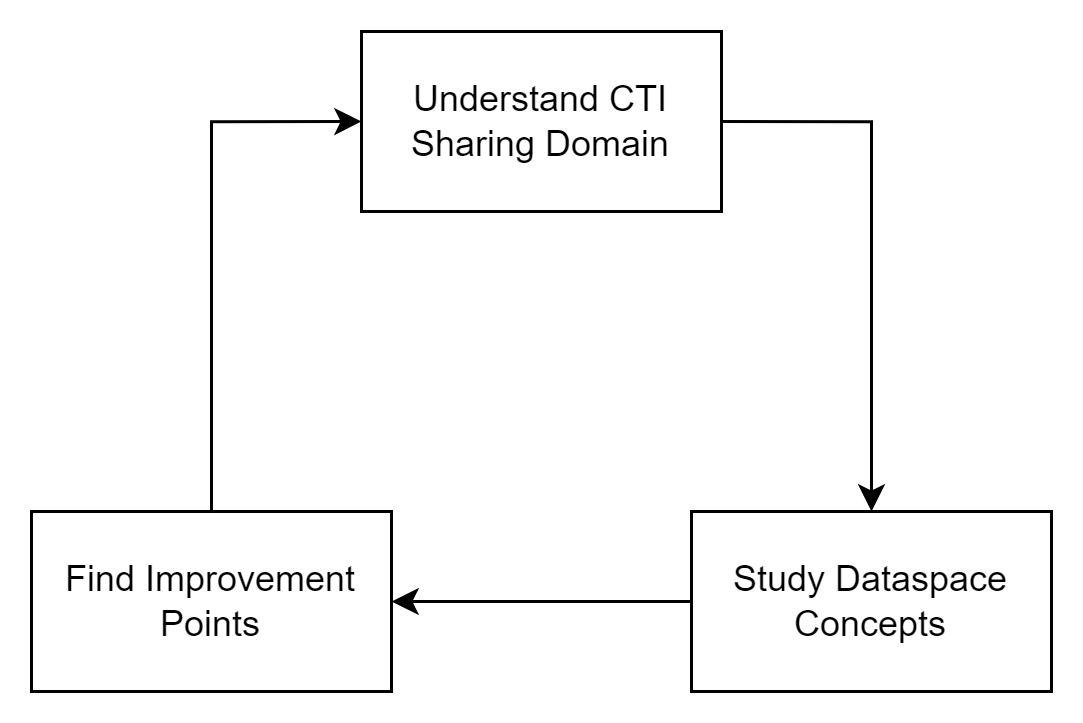
\includegraphics[width=0.8\textwidth]{diagrams/conceptual/methodology-p1}
    \caption{Inception Phase}
    \label{fig:inception-phase}
\end{figure}

In the second phase, construction, we will build an artifact based on the high-level design and requirements produced in the inception phase. To do so, we will follow the DSR design cycle. We will design the system, build prototypes, evaluate them, and find the shortcomings to improve it further. This phase is summarized in Figure \ref{fig:construction-phase}.

\begin{figure}[ht]
    \centering
    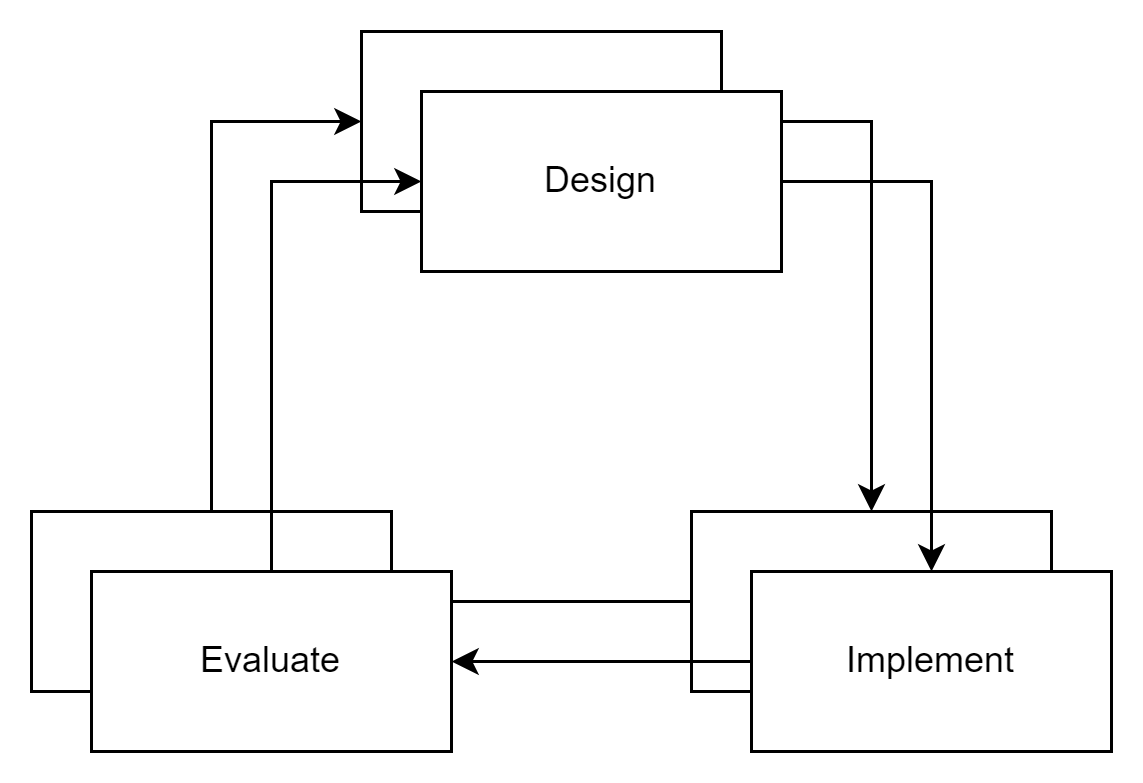
\includegraphics[width=0.8\textwidth]{diagrams/conceptual/methodology-p2}
    \caption{Construction Phase}
    \label{fig:construction-phase}
\end{figure}

\section{High Level Requirements}
In this section, we will try to understand the high-level requirements of a successful CTI sharing framework. We will justify the importance of each requirement based on real-world scenarios and the literature. We then try to understand which of these requirements are not met by the current systems. 

\subsection{R1 - Federation}
In this section, we will discuss the importance of federation in CTI sharing. We will try to understand the reason why a centralized repository is not practical and why current CTI sharing is dispersed, what problems does it pose to the participants, what is the importance of federation in CTI sharing, and what are the challenges in achieving it.

\subsubsection{Decentralized CTI Sharing}
In the current state of practice in CTI sharing, as mentioned in Section \ref{subsubsec:collaboration-communities}, the sharing of CTI is done in dispersed communities. Each community has its own set of rules, policies, and standards.
Organizations join these communities based on their interests and requirements.  National Institute of Standards and Technology (NIST) in its guide for CTI sharing \cite{johnson_guide_2016} provides a description of different sharing communities and a selection guide for organizations to choose the right community. There is no one-size-fits all solution for CTI sharing. There are communities around different geographic region, political boundary, industrial sector, business interest, or threat space (e.g., focused on phishing attacks) \cite{johnson_guide_2016}.
An important aspect is trust in the community. Organizations are more likely to share CTI with a community that they trust. This trust is built over time by the community's ability to protect the shared CTI and the community's ability to provide valuable CTI. It is often not possible to share CTI across communities due the policies or standards incompatibility which results in a fragmented CTI sharing landscape with siloed CTI repositories. 

\subsubsection{Incompatibile and Siloed CTI}
To reach their intelligence goals, organizations often need to join multiple communities \cite{johnson_guide_2016}. However, this puts a significant burden on the participants to manage and integrate the CTI from multiple sources due to several reasons. The lack of interoperability and different standards used by different communities, establishment of trust, and validating data quality are obstacles that participants should overcome \cite{zibak_cyber_2019}. 
Furthermore, lack of visibility across communities will hinder obtaining the full value from CTI sharing. For example, efforts to detect and mitigate a threat may be duplicated across communities \cite{zibak_cyber_2019}. Also, detection of advanced threats might not be possible because there was not enough information available to detect the threat. Another issue is the vendor lock-in problem, usually with the commercial providers, that is caused by the difficulty of moving from one CTI provider to another.

\subsubsection{Efforts to Achieve Federation}
To allievate the aforementioned issues a federated approach is required. In a federated approach, the CTI sharing communities are connected in a way that they can share CTI with each other while maintaining their autonomy. This requires a common set of standards, policies, and trust mechanisms that all the communities agree upon. There are some existing standardization efforts. The technical standards like STIX/TAXII (more information in background section \ref{subsubsec:cti-channels}) and the policy standards ISO/IEC27010, NIST, and ENISA report (ref. \ref{subsubsec:regulations}) are in this direction. 

\subsection{R2 - Interoperable}
To enable adoption of a common sharing framework by more community and participants, the framework should be easily integrated in existing systems and processes. Therefore, open, non-proprietary standards should be used for expressing the data, protocols for exchanging the data, and the legal framework to specify the policies attached to data should be used.

Existing Standards
\subsection{Trust and Data Sovereignty}
\subsection{Regulatory Compliance}
- why current systems are not enough -> Sovereginty

% 12 Pages
- Sovereignty by Decentralization
  promises of IDS
  usage control
  comparision

- CTI sharing more challenges more real world 
  3 pages
  real world scenarios

- High level requirements
say why each is important
    - security and trust
    - policy enforcement
    - sanitization
    - content quality (?)
    - being discoverable (?)
    - integration with existing systems (?)
    - information model

- Conceptual Approach
    say how each one is achieved in high level

- fn and nfn requirements

